\documentclass[paper=a4, fontsize=13pt]{article} 
\usepackage[top=1in, bottom=1in, left=1in, right=1in]{geometry}
\usepackage{amstext}
\usepackage{subfigure}
\RequirePackage{graphicx}
\RequirePackage{longtable,multirow,hhline,tabularx,array}
\usepackage[english]{babel} 
\RequirePackage{colortbl,booktabs}
\linespread{1.5}

\title{
\normalfont \normalsize
\huge Battle of Online and Offline Consumption: \\
Comparative Analysis of Amazon and Walmart Stocks
}
\author{Cai Yuzhu, Li Hongchi, Ning Xu, Xue Zheng}
\date{\normalsize\today}

\begin{document}
\maketitle
\section{Introduction}

\section{Data Processing}
Our research focuses on the daily log return of stocks of Amazon and Walmart. Start from January 3th, 2010 to December 30th, 2016. The sample size is 1761 and all of data are pulled from Wind Financial Terminal, which is the most widely used financial data system in China like Bloomberg Terminal in the U.S.. The formula we use to calculate the log return is
\[ r_t = ln(\frac{p_t}{p_{t-1}}) \times 100\% \]
where $p_t$ is the close price in day $t$ and $p_{t-1}$ is the close price in day {t-1}.

The descriptive statistics and time plot are shown as Table \ref{ds} and Firgure \ref{tp}.

\begin{table}[!htbp]
\caption{Descriptive Statistics}  
\centering  
\subtable[Amazon Stock]
{  
\begin{tabular}{ccccc}
  \toprule
  \rowcolor[gray]{.8}
Year & Sample & Mean(\%) & Sd(\%) \\ 
  \midrule
2010 & 251 & 0.1179 & 2.0591 \\ 
2011 & 252 & -0.0155 & 2.4337 \\ 
2012 & 250 & 0.1484 & 1.9656 \\ 
2013 & 252 & 0.1839 & 1.6947 \\ 
2014 & 252 & -0.0995 & 2.0677 \\ 
2015 & 252 & 0.3089 & 2.0582 \\ 
2016 & 252 & 0.0412 & 1.8682 \\ 
2010-2016 & 1761 & 0.0978 & 2.0323 \\ 
   \bottomrule
\end{tabular}
}  
\qquad  
\subtable[Walmart Stock]
{          
\begin{tabular}{ccccc}
  \toprule
  \rowcolor[gray]{.8}
Year & Sample & Mean(\%) & Sd(\%) \\ 
  \midrule
2010 & 251 & 0.0068 & 0.8782 \\ 
2011 & 252 & 0.0515 & 1.0469 \\ 
2012 & 250 & 0.0627 & 1.0309 \\ 
2013 & 252 & 0.0662 & 0.7749 \\ 
2014 & 252 & 0.0445 & 0.8367 \\ 
2015 & 252 & -0.1229 & 1.3191 \\ 
2016 & 252 & 0.0590 & 1.2030 \\ 
2010-2016 & 1761 & 0.0239 & 1.0297 \\ 
   \bottomrule
\end{tabular}
}
\label{ds} 
\end{table}  

\begin{figure}[!htbp]
\begin{minipage}[!htbp]{0.5\linewidth}
\centering
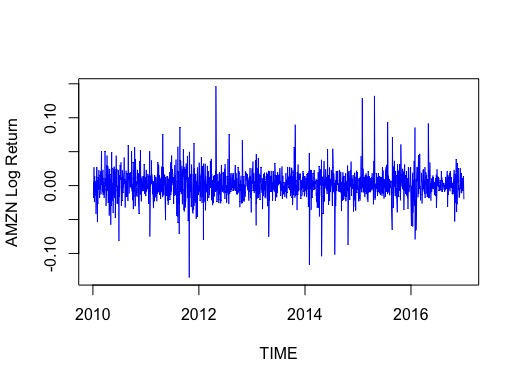
\includegraphics[scale = 0.45]{img/timeplot_AMZN}
\end{minipage}
\begin{minipage}[!htbp]{0.5\linewidth}
\centering
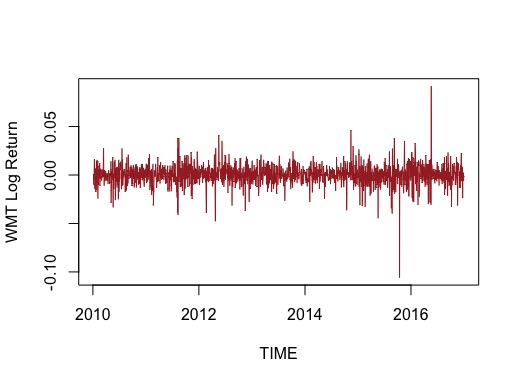
\includegraphics[scale = 0.45]{img/timeplot_WMT}
\end{minipage}
\caption{Timeplots of Amazon (Blue) and Walmart (Red) Stocks}
\label{tp}
\end{figure}

\section{Model Establishment}
\subsection{Model Specification}

\begin{figure}[!htbp]
\centering
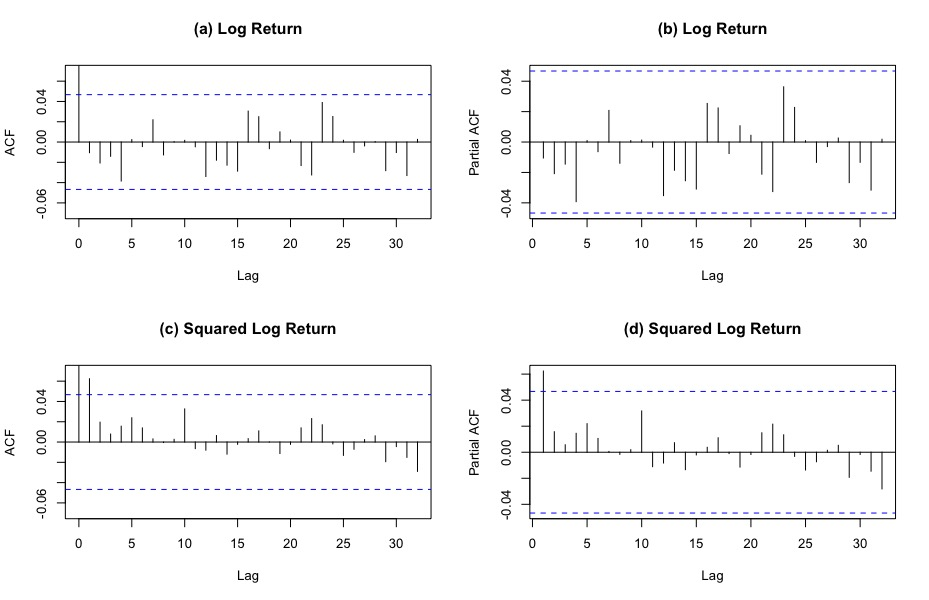
\includegraphics[scale = 0.7]{img/cf_AMZN}
\caption{ACF and PACF of Amazon Stock}
\label{cf_AMZN}
\end{figure}

\begin{figure}[!htbp]
\centering
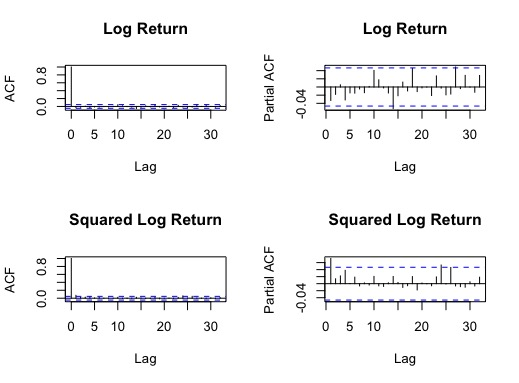
\includegraphics[scale = 0.7]{img/cf_WMT}
\caption{ACF and PACF of Walmart Stock}
\label{cf_WMT}
\end{figure}

\subsection{Mean Equation}
\subsection{Volatility Equation}

\section{Estimation}

\section{Model Checking}

\section{Prediction}

\section{Conclusion}

\section{Appendix}

\begin{thebibliography}{99}
\bibitem{1} hahahahahahahaha
\end{thebibliography}


\end{document}
